\documentclass[a4paper, 10pt]{article}
\date{12 February 2014}
\author{Shaun Schreiber \\ 16715128}
\title{Tutorial 2}
\usepackage{float}
\usepackage{tikz}
\usepackage{graphicx}
\usetikzlibrary{arrows, automata}
\begin{document}
\maketitle
\section*{Question 4a}
\begin{figure}[H]
\minipage{0.32\textwidth}
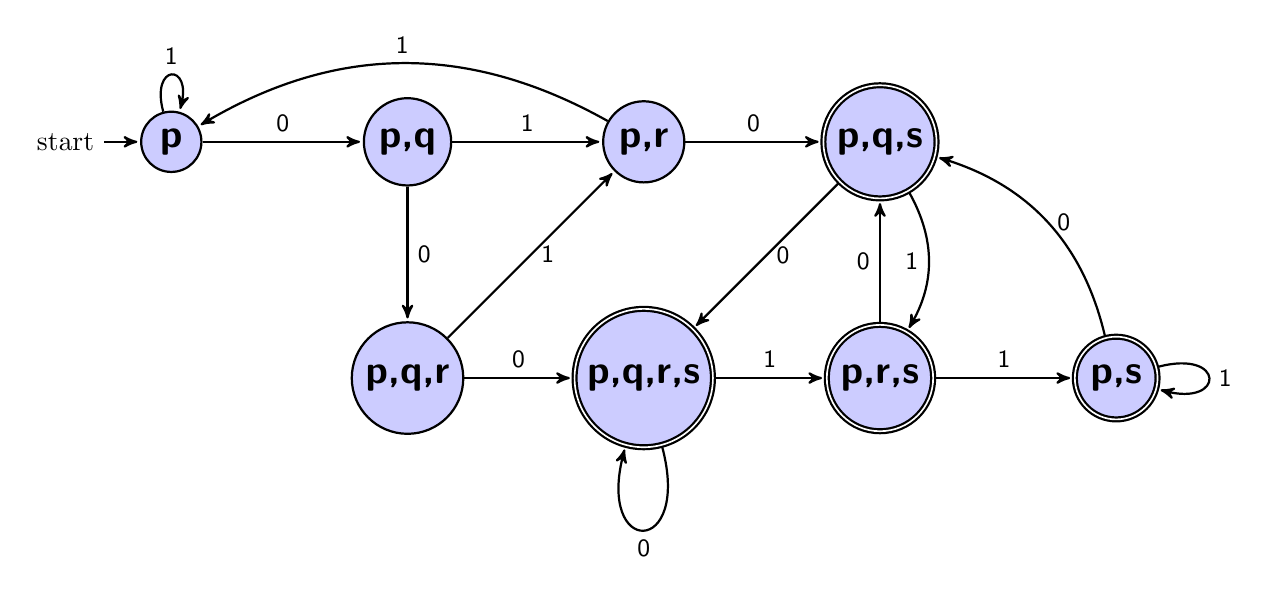
\begin{tikzpicture}[->,>=stealth',shorten >=1pt,auto,node distance=3cm,
  thick,main node/.style={circle,fill=blue!20,draw,font=\sffamily\Large\bfseries}]
  \node[main node, initial] (p) {p};
  \node[main node] (pq) [right of =p] {p,q};
  \node[main node] (pqr) [below of =pq] {p,q,r};
  \node[main node] (pr) [right of =pq]{p,r};
  \node[main node, accepting] (pqrs) [right of =pqr]{p,q,r,s};
  \node[main node, accepting] (pqs) [right of =pr] {p,q,s};
  \node[main node, accepting] (prs) [right of =pqrs] {p,r,s};
  \node[main node, accepting] (ps) [right of =prs] {p,s};
  \path[every node/.style={font=\sffamily\small}]
     (p)    edge[loop above] node [above]{1}(p)
	    edge node [above]{0}(pq)
     (pq)   edge node[above] {1}(pr)
            edge node [right] {0}(pqr)
     (pr)   edge[bend right] node [above]{1}(p)
	    edge node [above]{0}(pqs)
     (pqr)  edge node [right]{1}(pr)
	    edge node [above]{0}(pqrs)
     (pqrs) edge node [above]{1}(prs)
	    edge [loop below] node [below]{0}(pqrs)
     (pqs)  edge [bend left] node [left] {1} (prs)
            edge  node [right]{0}(pqrs)
     (prs)  edge node [above]{1}(ps)
	    edge node [left]{0}(pqs)
     (ps)   edge [loop right] node [right]{1}(ps)
	    edge [bend right] node [right]{0}(pqs);       
  \end{tikzpicture}
\endminipage\hfill
\end{figure}
\begin{table}[h!t]
\centering
\begin{tabular}{c | c c}
& 0 & 1 \\
\hline
\{$p$\} & \{$p, q$\} & \{$p$\} \\
\{$p, q$\} & \{$p, q, r$\} & \{$p, r$\} \\
\{$p, q, r$\} & \{$p, q, r, s$\} & \{$p, r$\} \\
\{$p, r$\} & \{$p, q, s$\} & \{$p$\} \\
\{$p, q, r, s$\} & \{$p, q, r, s$\} & \{$p, r, s$\} \\
\{$p, q, s$\} & \{$p, q, r, s$\} & \{$p, r, s$\} \\
\{$p, r, s$\} & \{$p, q, s$\} & \{$p, s$\} \\
\{$p, s$\} & \{$p, q, s$\} & \{$p, s$\} \\
\end{tabular}
\end{table}\section*{Question 4b}
\begin{figure}[H]
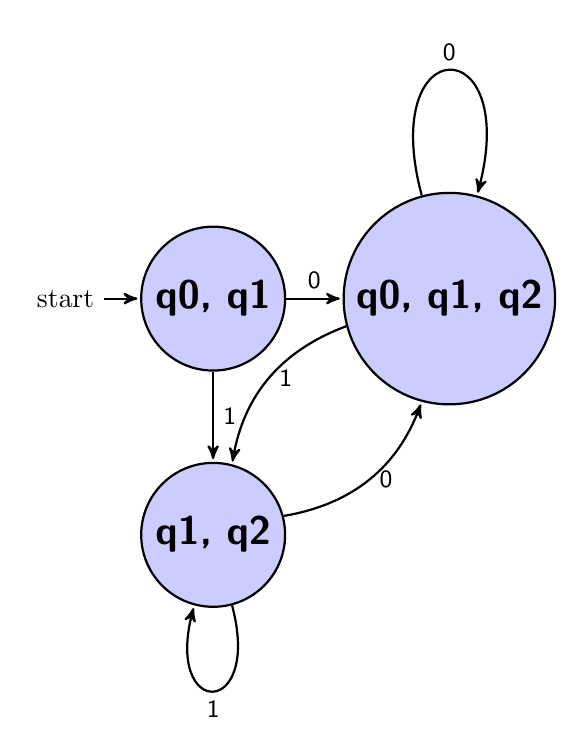
\begin{tikzpicture}[->,>=stealth',shorten >=1pt,auto,node distance=3cm,
  thick,main node/.style={circle,fill=blue!20,draw,font=\sffamily\Large\bfseries}]
  \node[main node, initial] (q0q1) {q0, q1};
  \node[main node] (q0q1q2) [right of =q0q1] {q0, q1, q2};
  \node[main node] (q1q2) [below of =q0q1] {q1, q2};
  \path[every node/.style={font=\sffamily\small}]
     (q0q1)   edge node [right]{1}(q1q2)
              edge node [above]{0}(q0q1q2)
     (q0q1q2) edge [loop above] node [above] {0}(q0q1q2)
	      edge [bend right] node [right] {1}(q1q2)
     (q1q2)   edge [loop below] node [below] {1}(q1q2)
	      edge [bend right] node [right]{0}(q0q1q2);
  \end{tikzpicture}
\end{figure}
\begin{table}[h!t]
\centering
\begin{tabular}{c | c c}
& 0 & 1 \\
\hline
\{$q0, q1$\} & \{$q0, q1, q2$\} & \{$q1, q2$\} \\
\{$q0, q1, q2$\} & \{$q0, q1, q2$\} & \{$q1, q2$\} \\
\{$q1, q2$\} & \{$q0, q1, q2$\} & \{$q1, q2$\} \\
\end{tabular}
\end{table}
\end{document}
